\documentclass[tikz]{standalone}
\usepackage{pgfplots}
\pgfplotsset{compat=1.15}
\usepackage{mathrsfs}
\usetikzlibrary{arrows,calc}
\usepackage{tkz-euclide}

\pagestyle{empty}

\definecolor{AngleClr}{rgb}{0,0.39215686274509803,0}
\definecolor{ShapeClr}{rgb}{0.6,0.2,0}

\begin{document}

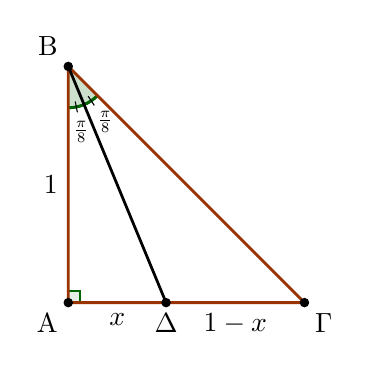
\begin{tikzpicture}[scale=.75]
\tkzSetUpLine[line width=1pt,color=black]
\tkzSetUpPoint[fill=black]

\tkzDefPoints{0/0/A,0/4/B,4/0/C}

\tkzDefLine[bisector](A,B,C) \tkzGetPoint{x}
\tkzInterLL(B,x)(A,C) \tkzGetPoint{D}

\tkzFillPolygon[fill=white](A,B,C)

\tkzMarkRightAngles[line width=0.5pt, size=.2,color=AngleClr,fill=AngleClr,fill opacity=0.1](B,A,C)

\tkzFillAngles[fill=AngleClr,size=.7,fill opacity=0.2](A,B,D D,B,C)
\tkzMarkAngles[line width=1pt,size=.7,color=AngleClr](A,B,D D,B,C)
\tkzMarkAngles[mark=|,mksize=2,line width=1pt,size=.7,color=AngleClr](A,B,D D,B,C)

\tkzDrawPolygon[color=ShapeClr](A,B,C)
\tkzDrawPoints[size=3](A,B,C,D)

\tkzDrawSegment(B,D)

\tkzLabelPoint[below left](A){$\rm A$}
\tkzLabelPoint[above left](B){$\rm B$}
\tkzLabelPoint[below right](C){$\rm \Gamma$}
\tkzLabelPoint[below](D){$\rm \Delta$}

\tkzLabelSegment[below](A,D){$x$}
\tkzLabelSegment[below](D,C){$1 - x$}
\tkzLabelSegment[left](A,B){$1$}

\tkzLabelAngles[scale=0.75,pos=1.5](A,B,D D,B,C){$\frac{\pi}{8}$}

\end{tikzpicture}

\end{document}
